\documentclass{article}
\usepackage[utf8]{inputenc}
\setlength{\parindent}{0em}
\setlength{\parskip}{1.4ex}
\usepackage[danish]{babel}
\usepackage[utf8]{inputenc}
\usepackage{graphicx}
\graphicspath{{pictures/}}
\usepackage{amsmath}
\usepackage{amsthm}
\newtheorem{theorem}{Sætning}

\title{DM500 Eksamensopgave}

\author{
	Thomas Urup Schjerlund\\
	\texttt{thsch20@student.sdu.dk}
	\and
	Tobias Klink Lehn\\
	\texttt{toleh20@student.sdu.dk}
	\and
	Philip Hayberg Thomsen\\
	\texttt{phtho20@student.sdu.dk}
	\and
	Sean Chrone Græns\\
	\texttt{segra20@student.sdu.dk}
}
\date{15. November 2020}

\begin{document}

\begin{titlepage}
\maketitle
\end{titlepage}

\section{Reeksamen DM527 Opg 1 - Tobias}
\begin{figure}[h]
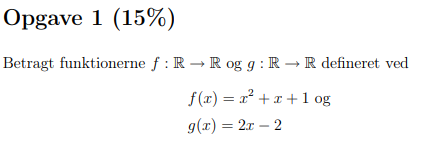
\includegraphics[scale=1]{Opgave1Formulering}
\end{figure}

\begin{figure}[h]
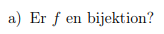
\includegraphics[scale=1]{opga}
\end{figure}
\textbf{Svar:}
For at en afbildning, $\phi: A \rightarrow B$ skal være bijektiv, kræves det, at funktionen både er \emph{injektiv} (one-to-one) og \emph{surjektiv} (onto.

\begin{theorem}
$f$ er injektiv, hvis $\forall x_1, x_2 \in Dm(f): x_1 \neq x_2 \rightarrow f(x_1) \neq f(x_2)$
\end{theorem}

Sagt på en anden måde, så skal det for alle værdier af x i definitionsmængden gælde, at x hvis to x-værdier er forskellige fra hinanden, så er deres funktionsværdier det også. Helt basalt vil det sige, at to x-værdier ikke kan dele en y-værdi.

Ved at indsætte $x_1$ og $x_2$ og sætte deres funktionsværdi lig hinanden, kan det afgøres hvorvidt det også betyder, at x-værdierne var ens til at starte med:
\begin{center}
\[f(x_1) = x_1^2 + x_1 + 1 \] 
\[ f(x_2)=x_2^2 + x_2 + 1 \] 
\begin{math}
f(x_1) = f(x_2) \Leftrightarrow x^2_1 + x_1 + 1 = x^2_2 + x_2 + 1
\end{math} 
\par
\begin{math}
\Rightarrow x^2_1 + x_1 = x^2_2 + x_2
\end{math} 
\end{center}

Definitionen på en injektiv funktion er, 




Jeg vil bare gerne have det her ind i TKL00OpgSkriv D:

\end{document}
